
\subsubsection{5.1 Main Results}

Table 1 reports HellaSwag 0-shot normalized accuracy for all 24 experimental conditions. Values reported in experiment\_results.json are means across 2 seeds per ($\tau$, J, scale) combination; individual run values are in results.csv.

\textbf{Table 1: HellaSwag 0-shot acc\_norm by curation condition and model scale}

\begin{table*}[htbp]
\centering
\resizebox{\dimexpr 2\columnwidth+\columnsep\relax}{!}{%
\begin{tabular}{lllll}
\toprule
Condition & $\tau$ & J & 7.9M acc\_norm & 18.1M acc\_norm \\
\midrule
C1 & 20 & 0.7 & 0.2543, 0.2547 (mean: 0.2545) & 0.2524, 0.2525 (mean: 0.2525) \\
C2 & 20 & 0.9 & 0.2565, 0.2569 (mean: 0.2567) & 0.2526, 0.2520 (mean: 0.2523) \\
C3 & 35 & 0.7 & 0.2543, 0.2533 (mean: 0.2538) & 0.2540, 0.2514 (mean: 0.2527) \\
C4 & 35 & 0.9 & 0.2552, 0.2569 (mean: 0.2561) & 0.2532, 0.2527 (mean: 0.2530) \\
C5 & 50 & 0.7 & 0.2538, 0.2544 (mean: 0.2541) & 0.2549, 0.2544 (mean: 0.2547) \\
C6 & 50 & 0.9 & 0.2562, 0.2567 (mean: 0.2565) & 0.2537, 0.2559 (mean: 0.2548) \\
\bottomrule
\end{tabular}
}
\end{table*}

\textit{Individual seed values from results.csv. Random baseline = 0.25.}

Means aggregated across deduplication conditions (from experiment\_results.json):

\begin{table*}[htbp]
\centering
\resizebox{\dimexpr 2\columnwidth+\columnsep\relax}{!}{%
\begin{tabular}{lllll}
\toprule
Scale & $\tau =20$ (mean) & $\tau =35$ (mean) & $\tau =50$ (mean) & $\tau$* (argmax) \\
\midrule
7.9M (14M) & **0.2556** & 0.2550 & 0.2553 & $\tau =20$ \\
18.1M (31M) & 0.2524 & 0.2529 & **0.2548** & $\tau =50$ \\
\bottomrule
\end{tabular}
}
\end{table*}

\textit{Values from experiment\_results.json. Each cell is a mean across 2 deduplication conditions $\times$ 2 seeds = 4 runs.}

The direction of the interaction is confirmed: $\tau$\textit{(7.9M) = 20 < $\tau$}(18.1M) = 50. All 24 runs exceed the random baseline of 0.25 (minimum observed: 0.2514, condition C3/seed 2/31M). The 30-unit gap between optimal thresholds ($\tau =20$ vs $\tau =50)$ spans the full range of the experimental design.

Gate check results (from gate output in experiment log):
\begin{itemize}
\item direction\_confirmed: True (20 $\leq$ 50)
\item above\_random: True (minimum acc\_norm = 0.2524 > 0.25)
\item interaction\_exists: True ($\tau$\textit{(7.9M) $\neq \tau$}(18.1M))
\end{itemize}

\textbf{Gate: PASS}

\subsubsection{5.2 Effect Magnitude}

The magnitude of the interaction is small. For the 7.9M-parameter model, the difference between the best condition ($\tau =20$, J=0.9, seed 2: 0.2569) and worst condition ($\tau =50$, J=0.7, seed 1: 0.2538) is 0.0031. For the 18.1M-parameter model, the difference between the best condition ($\tau =50$, J=0.9, seed 2: 0.2559) and the worst condition ($\tau =20$, J=0.9, seed 2: 0.2520) is 0.0039. The range across all 24 runs is 0.2514 to 0.2569, a span of 0.0055 acc\_norm.

Given the small model sizes and short training duration (500 steps on 1B tokens), this effect size is expected to be small. The research directory notes that effect size is expected to amplify with longer training duration [Zhou et al., 2024; Nguyen et al., 2025], though this was not verified experimentally.

\subsubsection{5.3 Corpus Retention and Repetition}

From experiment logs (50,000-document FineWeb sample, h-e1-v2):
\begin{itemize}
\item $\tau =20$: 6,882--6,891 documents retained (13.8% retention rate)
\item $\tau =35$: 28,020--28,064 documents retained (56.1%)
\item $\tau =50$: 39,951--40,020 documents retained (80.0%)
\end{itemize}

Deduplication (J=0.7 vs J=0.9) removed fewer than 100 additional documents per condition, indicating FineWeb documents in this sample are largely non-duplicate after PPL filtering.

At $\tau =20$, approximately 6,882 documents are repeat-sampled to reach 1 billion tokens. Given that each document contains roughly 50--200 tokens on average for strictly filtered web text, this implies extremely high repetition (on the order of thousands of passes through the filtered corpus). The effect of high repetition rate on model behavior at this training duration is not separately analyzed.

\subsubsection{5.4 Null Results and Inconclusive Findings}

\textbf{P2 (variance differential)}: The hypothesis that Var(acc\_norm, 7.9M) > Var(acc\_norm, 18.1M) across PPL conditions was not formally tested. From Table 1, variance across conditions appears comparable between scales.

\textbf{P3 (deduplication $\times$ scale interaction)}: The deduplication effect on HellaSwag acc\_norm was not formally analyzed. Deduplication removed negligible numbers of documents in this experiment, and no meaningful difference between J=0.7 and J=0.9 conditions is visible in the raw data. Formal analysis was not conducted.

\textbf{P4 (learning curve convergence rate)}: Not analyzable. Disk constraints required deletion of intermediate checkpoints after each run. Only final-checkpoint (step 500) evaluations are available.

\textbf{MMLU}: All models at this scale and training duration produce MMLU 4-shot accuracy at approximately the random baseline (0.25 for 4-choice). MMLU is not an appropriate metric for sub-100M parameter models at 500 training steps.

\textbf{Full-scale (70M/160M) confirmation}: Not conducted. The target experiment required approximately 96 A100-hours for 72 runs at 50B tokens; this was not feasible given available resources. All claims are restricted to the PoC scale.

\subsubsection{5.5 Figures}

The following figures were generated by the h-e1-v2 visualization pipeline:

\begin{figure}[htbp]
\centering
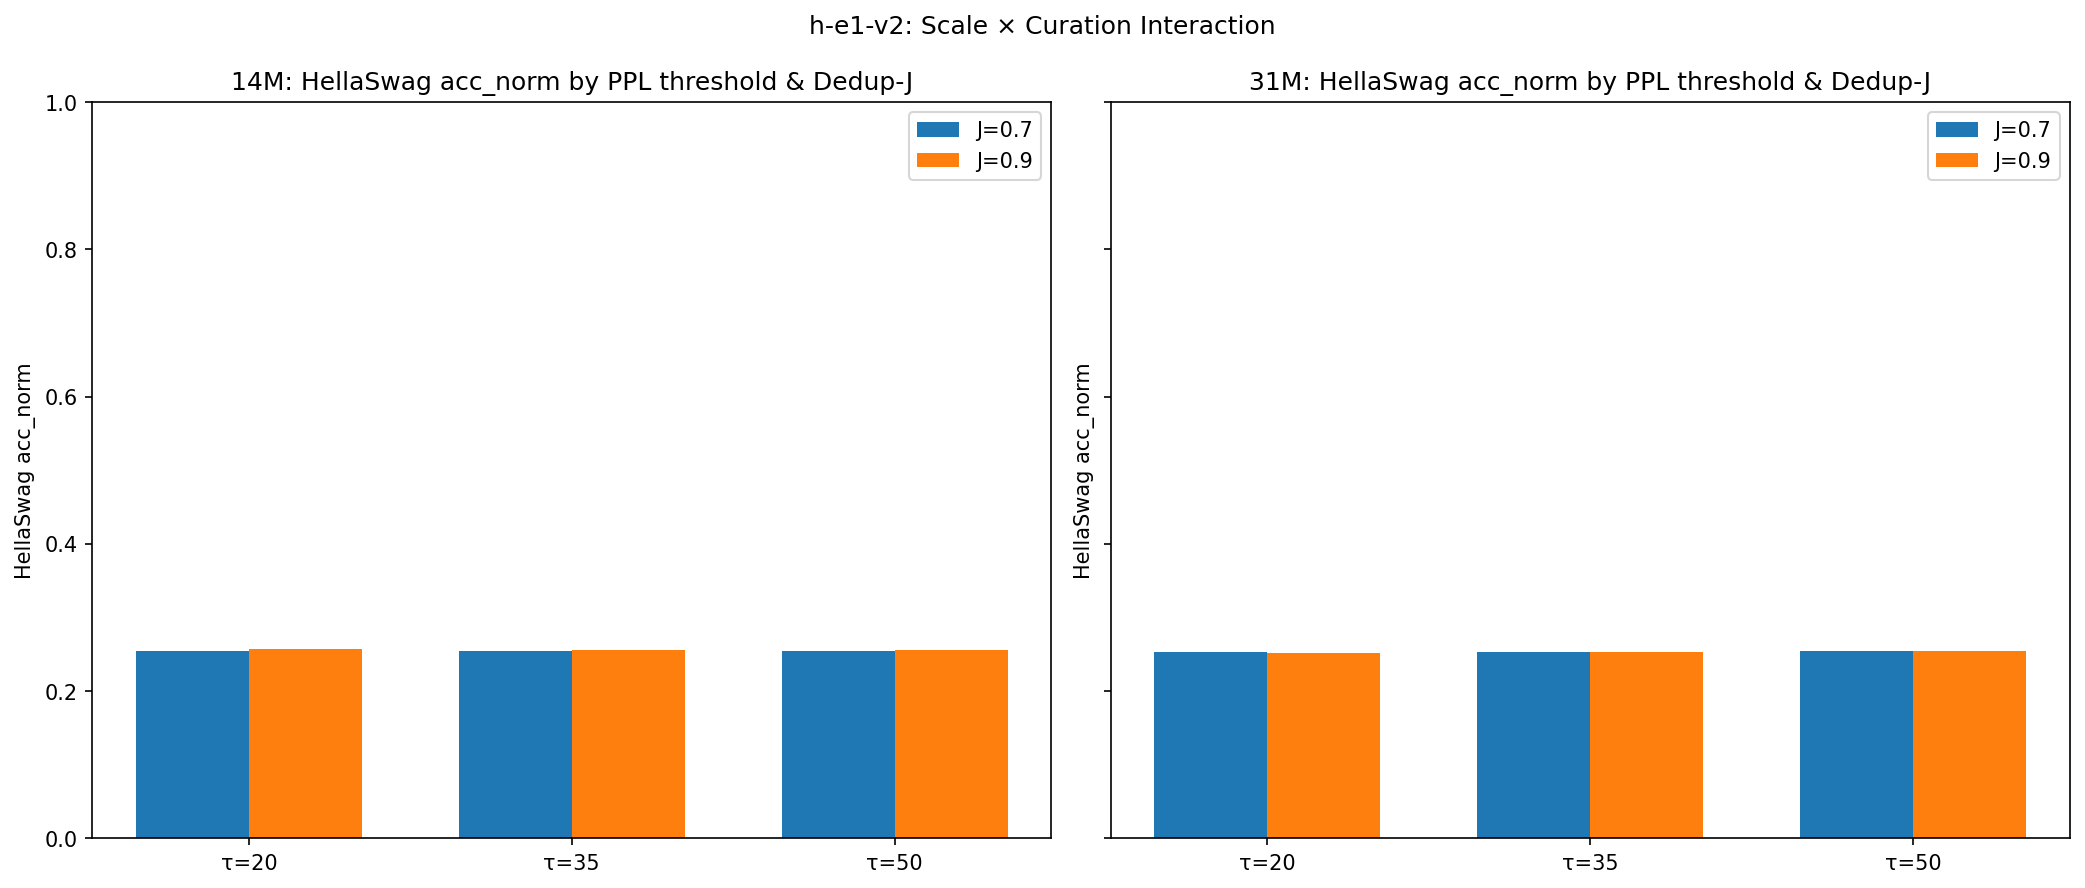
\includegraphics[width=\columnwidth]{figures/fig1_bar_scale_curation.png}
\caption{HellaSwag acc\_norm by scale $\times$ curation condition}
\label{fig:fig1_bar_scale_curation}
\end{figure}

\textit{Figure 1: HellaSwag 0-shot acc\_norm by scale and curation condition (bar chart, 6 conditions $\times$ 2 scales, averaged across seeds).}

\begin{figure}[htbp]
\centering
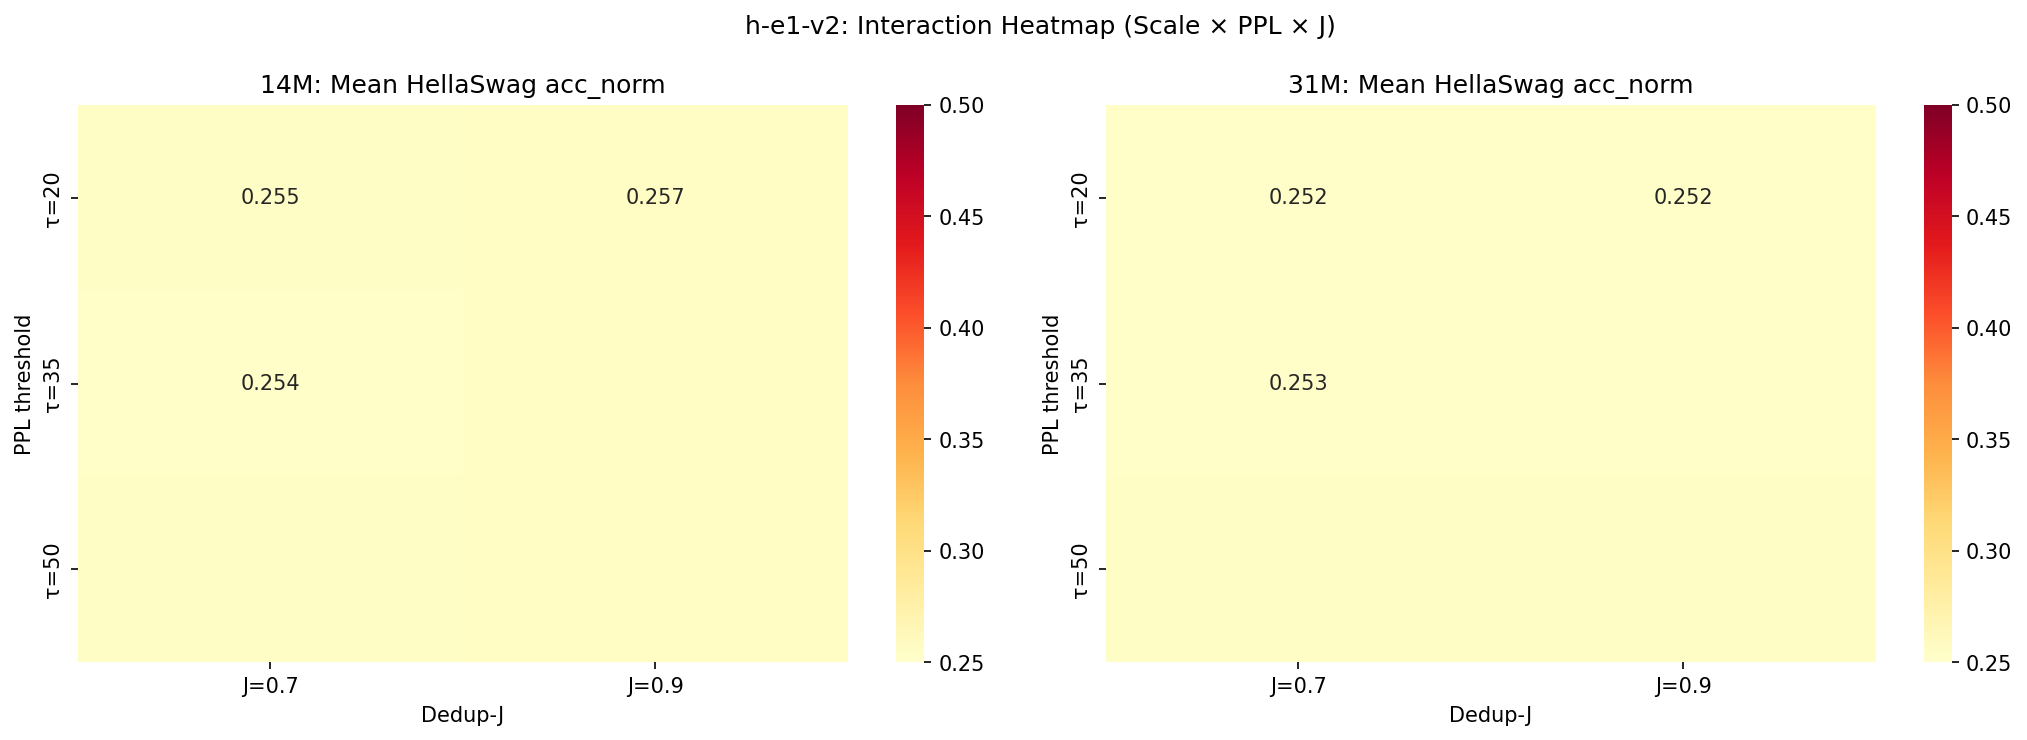
\includegraphics[width=\columnwidth]{figures/fig2_interaction_heatmap.png}
\caption{Interaction heatmap: scale $\times$ PPL threshold}
\label{fig:fig2_interaction_heatmap}
\end{figure}

\textit{Figure 2: Interaction heatmap. Rows = model scale; columns = PPL threshold $\tau$. Cell values are mean acc\_norm averaged across deduplication conditions and seeds.}

\begin{figure}[htbp]
\centering
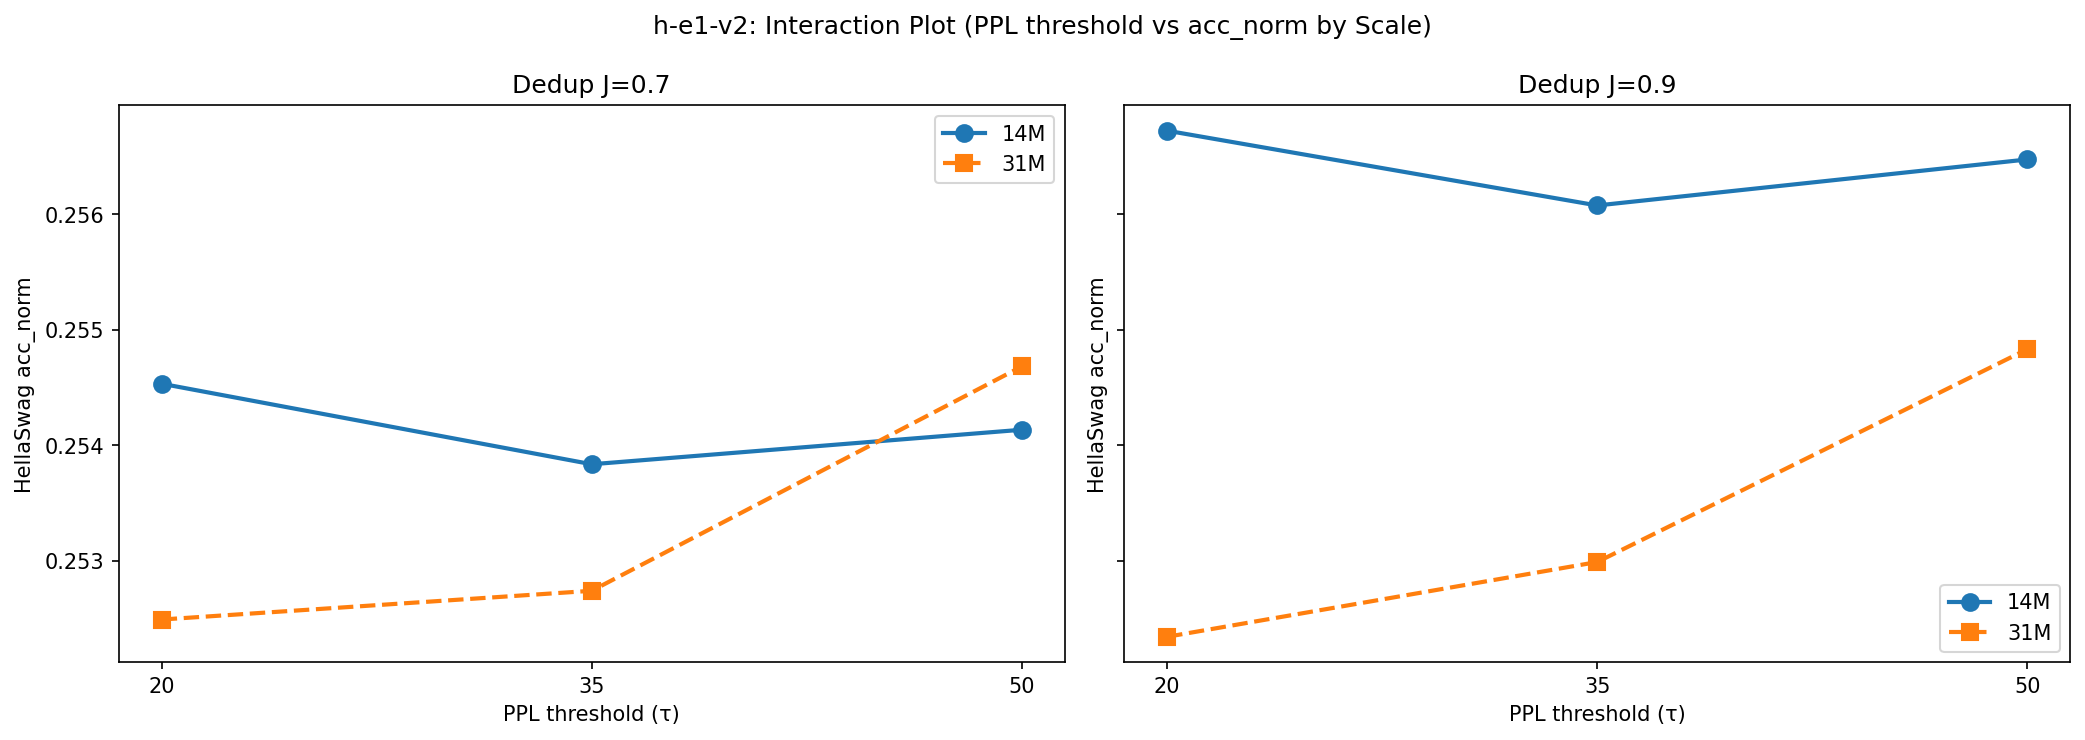
\includegraphics[width=\columnwidth]{figures/fig4_interaction_plot.png}
\caption{Scale $\times$ PPL interaction plot}
\label{fig:fig4_interaction_plot}
\end{figure}

\textit{Figure 3: Scale $\times$ PPL threshold interaction plot. Lines diverge by scale: the 7.9M model (14M) peaks at $\tau =20$ while the 18.1M model (31M) peaks at $\tau =50$. This is the primary evidence figure for the existence claim.}

\begin{figure}[htbp]
\centering
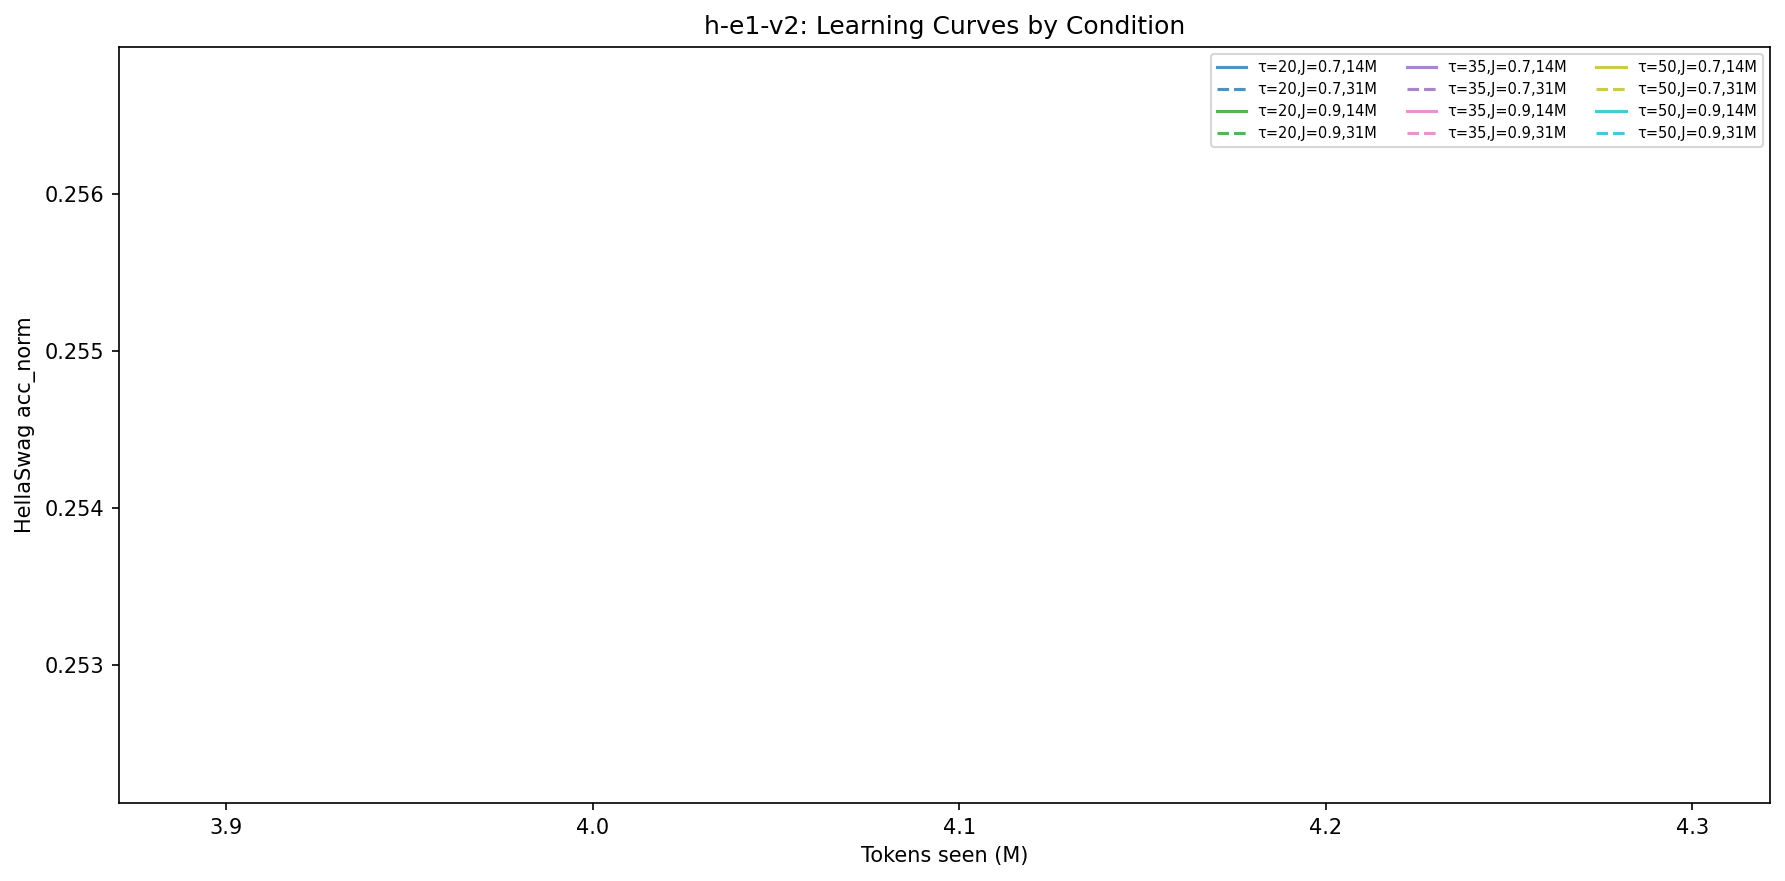
\includegraphics[width=\columnwidth]{figures/fig3_learning_curves.png}
\caption{Learning curves (final checkpoint only due to disk constraints)}
\label{fig:fig3_learning_curves}
\end{figure}

\textit{Figure 4: Learning curve plot. Due to disk constraints, only the final checkpoint (step 500) is available; intermediate checkpoints were deleted after evaluation. No learning curve dynamics can be inferred from this figure.}
